\documentclass[letterpaper,12pt]{article}
\usepackage{amsmath,amssymb,amstext,amsthm}
\usepackage[margin=1in,letterpaper]{geometry}
\usepackage{amsmath,amssymb}
\usepackage{algorithm}
\usepackage{algpseudocode}

\usepackage{graphicx}
\graphicspath{ {./imgs/} }

% Theorems numbered within sections
\newtheorem{theorem}{Theorem}[section]
% Lemmas share numbering with theorems
\newtheorem{lemma}[theorem]{Lemma}
% Propositions share numbering with theorems
\newtheorem{proposition}[theorem]{Proposition}
% Definitions numbered within sections
\newtheorem{definition}{Definition}[section]


\title{An introduction to lattice trapdoor}
\author{Ganyu Xu (g66xu)}
\date{Fall, 2023}

\begin{document}
\maketitle

\section*{Acknowledgement}
Thank you to Vinod Vaikuntanathan\cite{mit-cs294} and Daniele Micciancio\cite{ucsd-cse206a}, for publishing the lecture notes from MIT's CS294 and UCSD's CSE206A respectively, as well as Chris Peikert\cite{peikert2016decade} for his survey \textit{A decade of lattice cryptography}. The content from these lecture notes and survey inspired this project and provided a wealth of technical details that this project is based on.

\section{Introduction}
Trapdoor functions are the foundations of public-key cryptography. The most famous and popular trapdoor functions include the RSA trapdoor (it is easy to compute $m^e$ from $m$ and $e$ but difficult to recover $m$ from $m^e$ and $e$) and discrete log (it is easy to compute $g^x$ from $g, x$ but hard to recover $x$ from $g^x, g$). While these two trapdoors have been proved very successful over their decades of application, they are unfortunately both based on the hardness of integer factorization. Trapdoor functions based on other classes of hard problems have been of research interest since the early days of public-key cryptography, and they have gained increased attention efficient quantum factorization algorithm threatens the security guarantee of RSA and Diffie-Hellman schemes.

This project surveys a particular class of cryptographic trapdoor functions whose construction is based on lattices and whose security is based on the hardness of lattice problems such as the shortest vector problem (SVP) and the closest vector problem (CVP). In section 2, we will state these hard problems and discuss solutions including the nearest plane algorithm and the LLL basis reduction algorithm. In section 3, we will introduce the Goldreich-Golwasser-Halevi trapdoor construction and its applications.

\subsection{Notations and preliminaries}
Troughout this survey, vectors are denoted with bolded letters $\mathbf{v}$ while matrices are denoted by capital letters $B$. A basis $B \in \mathbb{Z}^{n \times b}$ is assumed to be full-rank integer matrix unless explicitly stated. The lattice generated by $B$ is denoted by $\mathcal{L}(B) = \{B\mathbf{x} \mid \mathbf{x} \in \mathbb{Z}^n \}$. The linear span of $B$ is denoted by $\operatorname{span}(B) = \{B\mathbf{x} \mid \mathbf{x} \in \mathbb{R}^n \}$.

Given a basis $B$, the Gram-Schmidt orthogonalization algorithm returns a second basis $B^\ast$ that spans the same linear space as $B$, but whose base vectors are pairwise orthogonal:

$$
\mathbf{b}_i^\ast = \mathbf{b}_i - \sum_{j<i}\mu_{i, j}\mathbf{b}_j^\ast,
\text{where} \; \mu_{i, j} = \frac{
    \langle \mathbf{b}_i, \mathbf{b}_j^\ast\rangle
}{\langle \mathbf{b}_j^\ast, \mathbf{b}_j^\ast\rangle}
$$

We define a projection of $\mathbf{x} \in \operatorname{span}(B)$ onto the set of orthogonalized basis $\{\mathbf{b}_j\}_{j=i}^n$ by the function $\pi_i$:

$$
\pi_i(\mathbf{x}) = \sum_{j \geq i} \frac{
    \langle \mathbf{x}, \mathbf{b}_j^\ast\rangle
}{
    \langle \mathbf{b}_j^\ast, \mathbf{b}_j^\ast \rangle
} \mathbf{b}_j^\ast
$$

It is easy to see that for $i = 1$, $\pi_i(\mathbf{x}) = \mathbf{x}$ is the identity function. Also, we can show that $\pi_i(\mathbf{b}_i) = \mathbf{b}_i^\ast$:

$$
\begin{aligned}
\pi_i(\mathbf{b}_i) 
&= \sum_{j\geq i}\frac{\langle \mathbf{b}_i, \mathbf{b}_j^\ast\rangle}{\langle \mathbf{b}_j^\ast, \mathbf{b}_j^\ast \rangle}\mathbf{b}_j^\ast \\
&= \sum_{j\geq i}\mu_{i, j}\mathbf{b}_j^\ast \\
&= \sum_{1 \leq j \leq n}\mu_{i, j}\mathbf{b}_j^\ast  - \sum_{j < i}\mu_{i, j}\mathbf{b}_j^\ast \\
&= \pi_1(\mathbf{b}_i) - \sum_{j < i}\mu_{i, j}\mathbf{b}_j^\ast \\
&= \mathbf{b}_i - \sum_{j < i}\mu_{i, j}\mathbf{b}_j^\ast \\
&= \mathbf{b}_i^\ast
\end{aligned}
$$

% \section{Preliminaries}
Throughout this survey, we denote vectors by bolded letters $\mathbf{v} \in \mathbb{Z}^n$. While lattices are defined as discrete subgroups over the real, in practice it is easier to exclusively work with integer lattices $\mathcal{L} \subseteq \mathbb{Z}^n$. We also exclusively work with full-rank lattices (whose basis $B \in \mathbb{Z}^{n \times n}$ is non-singular full-rank matrix).

There are a few preliminaries in the mathematics of lattices that are tremendously helpful with understanding the difficulty of hard lattice problems and with the trapdoor constructions based on these hard problems. We will discuss them in this chapter.

\subsection{Unimodular relationship}
First, we describe how two different basis of the same lattice relate to each other. This relationship plays a crucial role in the construction of the GGH trapdoor because the trapdoor scheme first generates a secret basis, then uses this relationship to generate a public basis of the same lattice.

> Let $\mathcal{L}(B)$ the lattice generated by the column vectors of matrix $B \in \mathbb{Z}^{n \times n}$, then $\mathcal{L}(B_1) = \mathcal{L}(B_2)$ if and only if there exists a unimodular matrix $U \in \mathbb{Z}^{n \times n}$ such that $B_1 = B_2U$

Here a unimodular matrix is a square matrix whose entries are integers and whose determinant is $\pm 1$. In the forward direction, if $B_1, B_2$ generate the same lattice, then each column of $B_1, B_2$ is a lattice point and can be represented using the other basis, which means that there exists integer matrix $U, V$ such that $B_1 = B_2U$ and $B_2 = B_1V$. With simple substitution, we find that $B_1 = B_2U = (B_1V)U$, so $B_1(I - VU) = 1$. Because $B_1$ is non-singular, it necessarily follows that $VU = 1$. By a symmetric argument, we also have $UV = 1$, which means that $V = U^{-1}$. we know $U, V$ to both be integer matrix, so their determinants both necessarily have to be $1$, thus proving that $U, V$ to both be unimodular matrix.

In the backward direction, if $B_1 = B_2U$ for some unimodular matrix $U$, then columns of $B_1$ are already points in the lattice generated by $B_2$, meaning that $\mathcal{L}(B_1) \subseteq \mathcal{L}(B_2)$. Because $U$ is unimodular, we also hve $B_2 = B_1U^{-1}$, where $U^{-1}$ is an integer matrix (in fact $U^{-1}$ is also unimodular), so by a symmetric argument we also have $\mathcal{L}(B_2) \subseteq \mathcal{L}(B_1)$. Therefore, $\mathcal{L}(B_1) = \mathcal{L}(B_2)$. $\blacksquare$

Knowing that two basis generate the same lattice if and only if they are related by a unimodular matrix, it is not hard to deduce that swapping columns, negating a column, and adding to a column an integer linear combination of all other columns all preserve the lattice generated by a matrix because each of the such action can be represented as a right multiplication by a unimodular matrix.

\subsection{Orthogonality and determinant}
The determinant of a lattice $\mathcal{L}(B)$ generated by a basis $B$ is the determinant of the matrix $B$. Knowing that two basis generate the same lattice if and only if they are related by a unimodular matrix (whose determinant is 1), it is not hard to see that the determinant is the same regardless of choice of basis. We can thus define the "determinant of a lattice" $\det(\mathcal{L})$ as an invariant of the lattice regardless of the choice of basis.

The determinant of a lattice can be geometrically interpreted as the "n-dimensional volume" of the fundamental parallelpiped, which is defined as a subset of $\mathbb{R}^n$:

$$
P(B) = B\cdot [0, 1)^n = \{\sum_{i=1}^n x_i\mathbf{b_i} \mid 0\leq x < 1 \}
$$

Note that it is often more convenient to "center" the fundamental parallelpiped around $\mathbf{0}$ and define it as $P(B) = B\cdot [-\frac{1}{2}, \frac{1}{2})^n$.

On the other hand, we are also concerned with "how orthogonal" the basis is. For that we define the orthogonality defect:

$$
\mathop{\text{ortho-defect}} = \frac{\prod_{i=1}^n \Vert \mathbf{b}_i \Vert}{\vert\det(B)\vert}
$$

Observe that if $B$ is also an orthogonal matrix whose columns are pair-wise orthogonal, then $\text{ortho-defect}(B) = 1$. Otherwise, the orthogonality defect of $B$ will be greater than 1. Geometrically, a greater orthogonality defect corresponds to a basis that is more "skewed".

Intuitively it is not hard to imagine that, for a fundamental parallelpiped with a fixed n-dimensional volume, the more skewed the basis is, the longer each basis will have to be to preserve the n-dimensional volume, and the further away the basis is from the origin. This is the principal observation on the hardness of the shortset vector problems and their siblings (such as the closest vector problem used in GGH's construction): \textbf{the longer, more skewed a basis is, the harder it is to find a short vector in the lattice}. It turns out that the gap in difficult of finding short vector between good (short, orthogonal) basis and bad (long, skewed) basis is exponential, and thus hard lattice problems pose provide an excellent foundation to build trapdoor functions on.
\section{Hard lattice problems and best known solutions}
We begin the discussion of hard lattice problems by defining two such problems. Unless otherwise specified, the Euclidean norm is used.

\begin{definition}
    Given a lattice $\mathcal{L}(B)$ spanned by basis $B$ and a norm $\Vert \cdot \Vert \rightarrow \mathbb{R}$, the \textbf{shortest vector problem} asks to find the shortest non-zero vector $\mathbf{v} \in \mathcal{L}(B)$
\end{definition}

The norm of the shortest non-zero vector is called the \textbf{minimum distance} and is denoted by $\lambda(\mathcal{L})$. Where the lattice is unambiguous we simply denote the minimum distance by $\lambda$.

\begin{definition}
    Given a lattice $\mathcal{L}(B)$, a norm, and some target vector $\mathbf{t}$ in the same vector space as the lattice, the \textbf{closest vector problem} asks to find a lattice point $\mathbf{v} \in \mathcal{L}$ that minimizes $\Vert \mathbf{t} - \mathbf{v}\Vert$
\end{definition}

There are two main parameters that affect the difficulty of SVP and CVP. The first is the number of dimensions $n$: the higher the number of dimension, the harder it is to find the shortest vector and/or the closest vector. The second is the orthogonality and/or the length of the basis. Intuitively, orthogonality and length are inversely related because the determinant of the lattice is invariant with respect to the choice of basis: higher orthogonality automatically implies shorter lengths. The more skewed the choice of basis, the more difficult it is to solve SVP/CVP.

\subsection{Reduced lattice basis}
At the time of this survey, the best algorithm for solving the (approximate) shortest vector problem is the LLL lattice basis reduction algorithm\cite{lenstra1982factoring}, attributed to Arjen Lenstra, Hendrik Lenstra, and László Lovász. The reduction algorithm transforms an input basis into an LLL-reduced form parameterized by a real number $\frac{1}{4} < \delta \leq 1$, where the first base vector of the reduced basis is an approximation of the shortest vector. Details of the actual algorithm for obtaining a reduced basis will be discussed in \ref{subsec:lllreduce}. Meanwhile, it is helpful to state the definition of the reduced basis and discuss its relationship to the shortest vector.

\begin{definition}
    A basis $B$ is $\delta$-LLL reduced if two conditions are satisfied
    \begin{enumerate}
    \item For all $j > i$, $\vert\mu_{j, i}\vert \leq \frac{1}{2}$
    \item For all $1 \leq i \leq n-1$, $\delta\Vert \pi_i(\mathbf{b}_i)\Vert^2 \leq \Vert\pi_i(\mathbf{b}_{i+1})\Vert^2$
\end{enumerate}
\end{definition}

The first condition will be discussed in details in \ref{subsec:nearestplane}. For now, we focus on the second condition, which gives us a description of how a reduced basis can be used to approximate the shortest vector.

\begin{theorem}
    If $B$ is $\delta$-LLL reduced basis, then
    $$
    \Vert \mathbf{b}_1 \Vert \leq \alpha^\frac{n-1}{2} \lambda
    $$
    where $\alpha = \frac{1}{\delta - \frac{1}{4}}$
\end{theorem}

In other words, the first base vector of a LLL-reduced basis is an approximation of the true shortest vector within an exponential factor.

\subsection{Babai's nearest plane algorithm}\label{subsec:nearestplane}
We denote the centered orthogonal parallelepiped as the following:

\begin{definition}
    Given basis $B$ and its Gram-Schmidt orthogonalization $B^\ast$, the \textbf{orthogonalized parallelepiped} is defined by

    $$
    \mathcal{C}(B^\ast) = \{
        B^\ast \mathbf{x} \mid \mathbf{x} \in [-\frac{1}{2}, \frac{1}{2})^n
    \}
    $$
\end{definition}

Babai's nearest plane algorithm, attributed to László Babai, is a recursive algorithm that can approximate the closest vector under a given basis to a target vector. More specifically, it returns a vector point $\mathbf{v}$ such that, if target vector is projected onto the orthogonalized basis, the projection is contained in $\mathbf{v} + \mathcal{C}(B^\ast)$. If the target vector is in the linear span of the basis, then the target vector itself is contained in $\mathbf{v} + \mathcal{C}(B^\ast)$.

\begin{algorithm}
\caption{NearestPlane}
\begin{algorithmic}[1]
    \If{$B$ is empty}
        \State return $\mathbf{0}$
    \EndIf 
    \State $B^\ast \leftarrow \text{GramSchmidt}(B)$
    \State $c \leftarrow \lfloor \frac{\langle\mathbf{t}, \mathbf{b}_n^\ast\rangle}{\langle\mathbf{b}_n^\ast, \mathbf{b}_n^\ast\rangle} \rceil$, where $\mathbf{b}_n^\ast$ is the last base vector in $B^\ast$
    \State return $c\mathbf{b}_n + \text{NearestPlane}([\mathbf{b}_1, \mathbf{b}_2, \ldots, \mathbf{b}_{n-1}], \mathbf{t} - c\mathbf{b}_n)$
\end{algorithmic}
\end{algorithm}


\begin{theorem}
    Given basis $B$ and target $\mathbf{t}$, denote the output of $\operatorname{NearestPlane}$ by $\mathbf{v} \leftarrow \operatorname{NearestPlane}(B, \mathbf{t})$, then for all $1 \leq i \leq n$:

    $$
    \frac{
        \langle
            \mathbf{t} - \mathbf{v}, \mathbf{b}_i^\ast
        \rangle
    }{
        \langle
            \mathbf{b}_i^\ast, \mathbf{b}_i^\ast
        \rangle
    } 
    \in [-\frac{1}{2}, \frac{1}{2})
        $$
    \end{theorem}

Intuitively, the inequality above states that the deviation of $\mathbf{t}$ from $\mathbf{v}$ is between $-\frac{1}{2}\mathbf{b}_i^\ast$ and $\frac{1}{2}\mathbf{b}_i^\ast$ in any of the chosen direction $\mathbf{b}_i^\ast$, which means that $\mathbf{t} - \mathbf{v}$ is indeed contained in the orthogonalized fundamental parallelpiped.

Babai's nearest plane algorithm is an essential component to the LLL lattice basis reduction algorithm. Specifically, the nearest plane algorithm is used to reduce the size of the basis vector so the first condition of the reduced basis (shown below) can be satisfied:

$$
\forall j<i, \vert\mu_{i, j}\vert \leq \frac{1}{2}
$$

The size reduction algorithm, which we will denote by $\operatorname{SizeReduce}$, takes a basis $B$ and returns a size-reduced basis $B^\prime$ such that the condition above is true.

\begin{algorithm}
\caption{SizeReduce}
\begin{algorithmic}[1]
    \For{$i \in \{2, 2, \ldots, n\}$}
        \State $\mathbf{v} \in \mathcal{L}([\mathbf{b}_1, \ldots, \mathbf{b}_{i-1}]) \leftarrow \operatorname{NearestPlane}([\mathbf{b}_1, \ldots, \mathbf{b}_{i-1}], \mathbf{b}_i - \mathbf{b}_i^\ast)$
        \State $\mathbf{b}_i \leftarrow \mathbf{b}_i - \mathbf{v}$
    \EndFor
\end{algorithmic}
\end{algorithm}

Recall the result of the nearest plane algorithm we know that:

$$
\forall j < i,
\frac{
    \langle
        \mathbf{b}_i - \mathbf{b}_i^\ast - \mathbf{v}, \mathbf{b}_j^\ast
    \rangle
}{
    \langle 
        \mathbf{b}_j^\ast, \mathbf{b}_j^\ast
    \rangle
} \in [-\frac{1}{2}, \frac{1}{2})
$$

Notice in the equation above, we have $\mathbf{b}_i^\ast \perp \mathbf{b}_j^\ast$ because $j < i$. We also have $\mathbf{b}_i - \mathbf{v}$ being the new value for $\mathbf{v}_i$ after the substitution. This means that after the substitution:

$$
\forall j < i,
\frac{
    \langle
        \mathbf{b}_i, \mathbf{b}_j^\ast
    \rangle
}{
    \langle
        \mathbf{b}_j^\ast, \mathbf{b}_j^\ast
    \rangle
} \in [-\frac{1}{2}, \frac{1}{2})
$$

The LHS of the equation above is exactly $\mu_{i,j}$. Thus we have satisfied the first condition of $\delta$-LLL reduced basis. In addition, because $\mathbf{v} \in \mathcal{L}([\mathbf{b}_1, \ldots, \mathbf{b}_{i-1}])$, the substitution $\mathbf{b}_i \leftarrow \mathbf{b}_i - \mathbf{v}$ is equivalent to adding onto the substituted basis a linear combination of other base vectors, which does not change the lattice.

%%%%% SECTION: LLL basis reduction algorithm %%%%%
\subsection{The LLL basis reduction algorithm}\label{subsec:lllreduce}
Applying the $\operatorname{SizeReduce}$ algorithm to a basis transforms it to satisfy the first condition of being $\delta$-LLL reduced. However, after the transformation, the second condition might not be satisfied everywhere, and we need to apply additional transformation to satisfy the second condition:

$$
\delta \Vert \pi_i(\mathbf{b}_i) \Vert^2 \leq \Vert \pi_i(\mathbf{b}_{i+1})\Vert^2
$$

It turns out that such transformation is rather simple: if there is some $i$ such that the condition above does not hold, then swapping $\mathbf{b}_i$ and $\mathbf{b}_{i+1}$ will make the pair satisfy the condition. To see that it works, denote the swapped basis vectors by $\mathbf{b}_i^\prime = \mathbf{b}_{i+1}$, $\mathbf{b}_{i+1}^\prime = \mathbf{b}_{i}$. First observe that the function $\pi_i: \mathbf{x} \mapsto \sum_{j\geq i}\frac{\langle \mathbf{x}, \mathbf{b}_j^\ast \rangle}{\langle \mathbf{b}_j^\ast, \mathbf{b}_j^\ast \rangle}\mathbf{b}_j^\ast$ is not changed after the swap because it is still projecting $\mathbf{x}$ onto the same set of orthogonal basis, and the set of orthogonal basis is unchanged by the swap.

If the condition does not hold, then $\delta\Vert\pi_i(\mathbf{b}_i)\Vert^2 > \Vert\pi_i(\mathbf{b}_{i+1})\Vert^2$, and we have

$$
\begin{aligned}
\delta \Vert\pi_i(\mathbf{b}_i^\prime)\Vert^2
&= \delta \Vert\pi_i(\mathbf{b}_{i+1})\Vert^2 \\
&< \delta \cdot \delta\Vert\pi_i(\mathbf{b}_i)\Vert^2 \\
&\leq \Vert\pi_i(\mathbf{b}_i)\Vert^2 \\
&= \Vert\pi_i(\mathbf{b}_{i+1}^\prime)\Vert^2
\end{aligned}
$$

We know that swapping columns preserves the lattice, so we can define a second algorithm $\operatorname{ColumnSwap}$ that takes a basis $B$ and transforms it into a second basis of the same lattice that satisfies the second condition of $\delta$-LLL reduced basis:

\begin{algorithm}
\caption{ColumnSwap}
\begin{algorithmic}[1]
    \For{$i \in \{1, 2, \ldots, n-1\}$}
        \If{$\delta\Vert\pi_i(\mathbf{b}_i)\Vert^2 > \Vert \pi_i(\mathbf{b}_{i+1}) \Vert^2$}
            \State $\mathbf{b}_i \leftarrow \mathbf{b}_{i+1}$
            \State $\mathbf{b}_{i+1} \leftarrow \mathbf{b}_{i}$
        \EndIf
    \EndFor
\end{algorithmic}
\end{algorithm}

It's easy to see that $\operatorname{ColumnSwap}$ always terminates in $n$ iterations, and upon termination, the transformed basis satisfies the second condition of being $\delta$-LLL reduced. Unforutnately, now the first condition might not hold everywhere, so we need to apply $\operatorname{SizeReduce}$ again.

Indeed, the LLL basis reduction algorithm repeatedly alternates between applying the two steps $\operatorname{SizeReduce}$ and $\operatorname{ColumnSwap}$ until the basis becomes $\delta$-LLL reduced. It's trivially true that if the algorithm terminates, the output is guaranteed to satisfy both conditions of being $\delta$-LLL reduced. It remains to show that, at least for $\delta < 1$, this algorithm terminates in polynomial time.

\begin{algorithm}
\caption{LLLReduce}
\begin{algorithmic}[1]
    \While{$B$ is not $\delta$-LLL reduced}
        \State $B \leftarrow \operatorname{SizeReduce}(B)$
        \State $B \leftarrow \operatorname{ColumnSwap}(B)$
    \EndWhile
\end{algorithmic}
\end{algorithm}

\begin{theorem}
    For $\delta < 1$, reducing a basis to $\delta$-LLL reduced form takes polynomial time
\end{theorem}
\begin{proof}
    To prove that $\operatorname{LLLReduce}$ will terminate in polynomial time, we define a positive integer quantity associated with a basis and show that each iteration of $\operatorname{SizeReduce}$ and $\operatorname{ColumnSwap}$ reduce this quantity by $\delta$.

    Recall that although determinant is not defined for non-square matrix, it is defined for (sub)lattice generated by sub-basis $B_k = [\mathbf{b}_1, \mathbf{b}_2, \ldots, \mathbf{b}_k] \in \mathbb{Z}^{n \times k}$ where $1 \leq k \leq n$:

    $$
    \det(\mathcal{L}(B_k)) = \prod_{i=1}^k \Vert \mathbf{b}_i^\ast \Vert = \sqrt{B_k^\intercal B_k}
    $$

    From the definition above we can see that the square of the determinant of a lattice generated by integer basis is an integer. 

    We define the "potential" of a full-rank basis $B = [\mathbf{b}_1, \mathbf{b}_2, \ldots, \mathbf{b}_n]$ by the product of determinants of sub-lattices generated by sub-basis $B_1, B_2, \ldots, B_n$:

    $$
    \mathcal{D} = \prod_{k=1}^n \det(\mathcal{L}(B_k))^2
    $$

    $\mathcal{D}$, being a product of integers, is itself an integer.

    First observe that in $\operatorname{SizeReduce}$, the basis vector is changed by subtracting a linear combination of basis vectors before the changed basis vector. This means that after $\operatorname{SizeReduce}$, each of $B_k$ for $1\leq k \leq n$ still generates the same lattice, and the determinant of that lattice remains unchanged. In other words, $\operatorname{SizeReduce}$ does not change the value of $\mathcal{D}$.

    Second, for $k < i$, swapping column $\mathbf{b}_i$ with $\mathbf{b}_{i+1}$ does not affect the lattice generated by the partial basis $B_k$ because $B_k = \{\mathbf{b}_1, \ldots, \mathbf{b}_{i-1}\}$ does not contain the swapped columns anyways. On the other hand, for $k > i$, swapping column $\mathbf{b}_i$ with $\mathbf{b}_{i+1}$ also does not affect the lattice generated by the partial basis $B_k$ because it contains both of the swapped column, and swapping column preserves the lattice.

    Therefore the only change to $\mathcal{D}$ when swapping $\mathbf{b}_i$ with $\mathbf{b}_{i+1}$ comes from the factor $\det(\mathcal{L}(B_i))$. Denote the potential of the basis $B$ after the swap by $\mathcal{D}^\prime$ then:
    
    $$
    \frac{\mathcal{D}}{\mathcal{D}^\prime} = \frac{
        \det(\mathcal{L}([\mathbf{b}_1, \mathbf{b}_2, \ldots, \mathbf{b}_{i-1}, \mathbf{b}_{i}]))^2
    }{
        \det(\mathcal{L}([\mathbf{b}_1, \mathbf{b}_2, \ldots, \mathbf{b}_{i-1}, \mathbf{b}_{i+1}]))^2
    } = \frac{\Vert\mathbf{b}_i^\ast\Vert^2}{\Vert\pi_i(\mathbf{b}_{i+1})\Vert^2}
    = \frac{\Vert\pi_i(\mathbf{b}_{i})\Vert^2}{\Vert\pi_i(\mathbf{b}_{i+1})\Vert^2}
    $$

    Because we only swap when $\delta \Vert \pi_i(\mathbf{b}_i) \Vert^2 > \Vert \pi_i(\mathbf{b}_{i+1}) \Vert^2$, the quotient above satisfies:

    $$
    \frac{\mathcal{D}}{\mathcal{D}^\prime} 
    = \frac{\Vert\pi_i(\mathbf{b}_{i})\Vert^2}{\Vert\pi_i(\mathbf{b}_{i+1})\Vert^2}
    > \frac{1}{\delta}
    $$

    Which implies $\mathcal{D}^\prime < \delta \mathcal{D}$.

    Notice that in the relationship above, the second condition of being $\delta$-LLL reduced is violated if and only if $\mathcal{D}^\prime < \delta\mathcal{D}$. This means that when $\mathcal{D}^\prime \geq \delta\mathcal{D}$, the second condition will hold. Indeed, when the potential converges, the algorithm terminates, and since each iteration reduces the potential by $\delta$, we can deduce that the algorithm will terminate in $O(\log_{\frac{1}{\delta}}\mathcal{D})$ time.
\end{proof}

\section{The Goldreich-Goldwasser-Halevi trapdoor}

One class of constructing lattice trapdoor uses a pair of public and secret basis for the same lattice. Since the two basis generate the same lattice, they are equally good at mapping integer coordinates into a lattice point. On the other hand, the secret basis is very "good" and can be used to efficiently find the closest lattice point, but the public basis is very "bad" at recovering the closest lattice point.

One of the earliest instances of such class of lattice trapdoor is proposed by Goldreich, Goldwasser, and Halevi in their 1997 paper \textit{"Public-key cryptosystem from lattice reduction problem"}\cite{goldreich1997public}. At a high level, the trapdoor is parameterized by three items: a "bad" basis $B$, a "good" basis $R$, and an error bound $\sigma$. In the forward direction, the function maps a pair of lattice coordinate $\mathbf{v} \in \mathbb{Z}^n$ and a small error vector $\mathbf{e} \leftarrow \{ -\sigma, \sigma \}^n$ to $\mathbf{x} = B\mathbf{v} + \mathbf{e} \in \mathbb{R}^n$. If the parameters are generated correctly, then the closest lattice point in $\mathcal{L}(B)$ is exactly $B\mathbf{v}$.

Inverting the function involves recovering the integer coordinate $\mathbf{v}$ (or the error vector $\mathbf{e}$, since recovering one of them automatically gives you the other). However, the inversion is exactly the closest vector problem (CVP), and should be hard if $B$ is a sufficiently bad basis. On the other hand, since $R$ is a good basis, finding the closest vector point should be "easy" if we have $R$.

From here, GGH '97 proposed a public-key cryptosystem as well as a digital signature scheme that uses such a trapdoor construction, and the security of the two schemes naturally rest on the hardness of the underlying hard lattice problem.

\subsection{The trapdoor scheme}
The GGH trapdoor scheme contains four components:

\begin{enumerate}
    \item \textbf{Parameter generation} The main security parameter in this scheme is the number of dimensions $n$ of the lattice. In the original paper, the authors claimed $n \approx 150$ is sufficient for making inverting the function without the private basis hard and $n \approx 250$ should be a safe choice for the foreseeable future.
    \item \textbf{Key generation} First generate the "good" basis $R \in \mathbb{R}^{n \times n}$, then apply some (unimodular) transformation to $R$ to obtain the "bad" basis $B$. The error bound $\sigma > 0 \in \mathbb{R}$ is dependent on the choice of $R$ and the choice of "probability of inversion error" $\epsilon >= 0$, which will be discussed in a later section.
    \item \textbf{Forward evaluation} $f_{B}(\mathbf{v}, \mathbf{e}) = B\mathbf{v} + \mathbf{e}$, where $\mathbf{v} \in \{-n, \ldots, n\}^n$ and $\mathbf{e} \in \{-\sigma, \sigma\}$. According to the authors, the choice of bounds for values of $\mathbf{v}$ is arbitrary and not a significant contributor to the overall security of the scheme.
    \item \textbf{Inversion} Denote the output by $\mathbf{x} = f_{B}(\mathbf{v}, \mathbf{e})$, first attempt to recover the integer coordinate $\mathbf{v} \leftarrow B^{-1}R\lfloor R^{-1}\mathbf{x} \rceil$. From here it is trivial to recompute the lattice point $B\mathbf{v}$ and recover the error term $\mathbf{e} = \mathbf{x} - B\mathbf{v}$.
\end{enumerate}

\subsection{Correctness of trapdoor inversion}
Without the error term, the function $f_B: \mathbf{v} \mapsto B\mathbf{v}$ is trivially invertible with either choice of the basis. However, with a non-zero the error term, the quality of the basis makes a substantial difference in how much error can be added before the points can no longer be recovered.

Observe the calculation used for recovering the integer coordinate $\mathbf{v}$:

$$
\begin{aligned}
\lfloor R^{-1}\mathbf{x} \rceil &= B^{-1}R\lfloor R^{-1}(B\mathbf{v} + \mathbf{e})\rceil \\
&= B^{-1}R\lfloor R^{-1}B\mathbf{v} + R^{-1}\mathbf{e}\rceil
\end{aligned}
$$

Since $R, B$ are related by a unimodular matrix and $\mathbf{v}$ is an integer vector, $R^{-1}B\mathbf{v}$ is an integer vector and can be moved out of the "rounding" operator:

$$
\begin{aligned}
\lfloor R^{-1}\mathbf{x} \rceil &= B^{-1}RR^{-1}B\mathbf{v} + B^{-1}R\lfloor R^{-1}\mathbf{e}\rceil \\
&= \mathbf{v} + B^{-1}R\lfloor R^{-1}\mathbf{e} \rceil
\end{aligned}
$$

Since $B^{-1}R$ is also a unimodular matrix, we can conclude that the equation above is successful at recovering the original coordinate if and only if $R^{-1}\mathbf{e} = \mathbf{0}$.

To guarantee that inversion error never happens, we can bound the error term $\sigma > 0$ by $\frac{1}{2\rho}$, where $\rho$ is maximal $L_1$ norm among the rows of $R^{-1}$. This bound is excessively conservative, however, and we might want to relax the bound to enhance the security of the trapdoor scheme (larger error terms makes it harder to invert the function using only the public basis). The authors provided one such relaxation based on the Hoeffding inequality. This relaxation is stated as follows

$$
P(\text{inversion error}) \leq 2n \cdot \exp(-\frac{1}{8\sigma^2\gamma^2})
$$

Where $\gamma = \sqrt{n} \cdot \max(L_\infty \text{ norm of rows of } R^{-1})$. Simple reorganization of inequality shows that to bound the inversion error by $\epsilon$, the error term will be bounded by $\sigma \leq (\gamma\sqrt{8\ln{2n/\epsilon}})^{-1}$.

\subsection{Generating the pair of basis}
The authors described two ways of generating the private basis. The first way is to sample each coordinate of $R \in \mathbb{R}^{n \times n}$ from a uniform distribution on $\{-l, -l + 1, \ldots, l-1, l\}$, where according to the authors, the value of the bound $l$ has negligible impact on the quality of the generated basis (the authors chose $\pm 4$ in their implementation). A second method is to first generate a square lattice $L(kI)$ for some positive integer $k$, then add a small amount of noise $R^\prime \in \{-l, \ldots, l\}^{n \times n}$. With this method of sampling the private basis, it is important to balance the choice of values between $k$ and $l$, where a larger $k$ value gives a more orthogonal basis, but also weakens the security of the trapdoor function by making it easier to reduce the public basis into a short, orthogonal basis using basis reduction algorithm.

The authors also described two methods for generating the public basis $B$ from the private basis. The first method is to directly generate random unimodular matrix $T$ and set $B = TR$, then repeat until satisfactory. A second method is to repeatedly apply column mixing, where at each mixing a column of $R$ is chosen, and a linear combination of all other columns is added to the chosen column.

Mathematically, the two methods are equivalent. However, in implemenetation, we would like the values of $B$ to be smaller for space efficiency while maintaining sufficient security so that the function cannot be easily inverted using the public basis alone and so that $B$ cannot be easily reduced using basis reduction algorithm. The authors preferred column mixing for requiring less computation and for producing public basis $B$ with smaller values.

Unfortunately, there is no known rigorous description of how skewed $B$ needs to be for the trapdoor function to be secure. The authors relied on experimental methods and determined that for $n \approx 100$, $2n$ steps of column mixing is enough to render LLL basis reduction ineffective at meaningfully improving the quality of the public basis $B$.

In 2001, Daniele Micciancio proposed to generate the public basis by computing the Hermite normal form of the private basis\cite{micciancio2001improving}. From a high level, Hermite normal form provides an optimal security guarantee because it is an invariant of the lattice, so a public basis computed from the Hermite normal form is guaranteed to give exactly zero information about the private basis. We will not discuss the details of Hermite normal in this survey.

\subsection{Security of the trapdoor}
It is easy to see that if an adversary can invert the trapdoor function without with only the public basis, then the adversary has found the closest vector $\mathbf{v} \in \mathcal{L}$ to the target $\mathbf{x}$. In other words, the adversary can solve the (approximate) closest vector problem.

As discussed in section 2, a polynomial-time LLL basis reduction algorithm only provides an approximation within an exponential factor; while it is possible to achieve approximation within a polynomial factor, the basis reduction algorithm is no longer guaranteed to run in polynomial time. In addition, the complexity of both LLL basis reduction and Babai's nearest plane algorithm scales exponentially with the security parameter $n$, and in experimental settings, the authors found that for $n \geq 100$ the workload for these algorithms starts becoming infeasible. The authors speculated that $n = 250$ should provide sufficient security in future production usage.


\subsection{Public key cryptosystem}
The authors of the GGH paper presented a public key cryptosystem that makes direct usage of the trapdoor \cite{goldreich1997public}. The main security parameter is $n$ the number of dimension of the lattice. The secret key is the short, orthogonal basis $R$ generated by applying a small amount of noise to a truly orthogonal basis. The public key is the long basis $B$ generated by applying column mixing to $R$. The encryption function is exactly the evaluation of the trapdoor, and the decryption function is the inversion of the trapdoor.

What remains is the question of "where to encode the message", for which the authors discussed a few options:

\begin{enumerate}
    \item Use a generic encoding that takes advantage of the hard-core bits of the one-way function, although this encoding is inefficient (it only encodes $\log{n}$ bits at a time), and it does not take advantage of any specific features of the trapdoor construction itself
    \item Directly encode the message into a lattice point $\mathbf{v}$. However, this scheme is insecure because an adversary can compute $B^{-1}\mathbf{c} = \mathbf{v} + B^{-1}\mathbf{e}$, where $B^{-1}\mathbf{e}$ might not be big enough to obscure all information about $\mathbf{v}$, which means this adversary can obtain partial information about the message
    \item Encode the message into the least significant bits of each entry of $\mathbf{v}$ and choose all other bits randomly. The authors argued that with appropriate choice of probability distribution for the error term $\mathbf{e}$, no polynomial-time adversaries will be able to distinguish the parity of the entries of the ciphertext from truly random, thus achieving IND-CPA security.
\end{enumerate}

Later Micciancio also proposed to encode the message in the error term $\mathbf{e}$, and instead chooses the lattice point $\mathbf{v}$ at random \cite{micciancio2001improving}. However, this scheme is not trivial because special care is needed for security requirement, and we also have the problem of a lattice being a countably infinite set, making defining probability distribution a non-trivial problem.

\subsection{Digital signature}
The GGH trapdoor is also suitable for a digital signature: the message is an arbitrary point in the linear span of the good basis, and the signature is the (approximate) closest lattice point, which can be efficiently computed using the good basis $R$. The verifier checks that the signature is valid by first using the public basis to verify that the signature is a lattice point, then computing the norm between the signature and the message to check that the distance is sufficiently small.
\section{Cryptanalysis of GGH signatures}
While the GGH trapdoor is based on CVP, a known hard lattice problem, the public-key cryptosystem and the signature schemes proposed by GGH in their original form are not given formal security proofs. Indeed, in 1999 the proposed public-key cryptosystem was cryptanalyzed by Phong Q. Nguyen \cite{nguyen1999cryptanalysis}, who successfully solved the GGH encryption challenges posed by the original authors. Later, Nguyen and Oded Regev published cryptanalysis of the GGH signature scheme \cite{nguyen2006learning}, which exploited the signature scheme's design flaws that caused message-signature pairs to leak information about the secret key.

In this section we will discuss the cryptanalysis of the GGH signature scheme by first summarizing the key results from Nguyen and Regev, then provide an implementation that simulate the key-recovery attack.

\subsection{Learning a hidden parallelepiped}
As Nguyen and Regev pointed out, the main weakness of the GGH signature scheme lies in the fact that messages are hashed uniformly into (a finite subset) of $\mathbb{Z}^n$ and each signature is exactly the unique lattice point $\mathbf{v} \in \mathcal{L}(R)$ (where $R$ is the secret basis) whose centered fundamental parallelepiped $\mathbf{v} + \mathcal{C}(R) = \{\mathbf{v} + R\mathbf{x} \mid \mathbf{x} \in [-\frac{1}{2}, \frac{1}{2})\}$ contains the hashed message. This means that for each message-signature pair $(\mathbf{m}, \mathbf{\sigma})$, their difference $\mathbf{m} - \mathbf{\sigma}$ is a uniform sample of the centered fundamental parallelepiped $\mathcal{C}(R)$. The cryptanalysis of the GGH signature scheme is thus an algorithm that approximates the basis spanning $\mathcal{C}(R)$, which Nguyen and Regev termed the \textit{hidden parallelepiped problem} (HPP).

\begin{figure}[h]
    \centering
    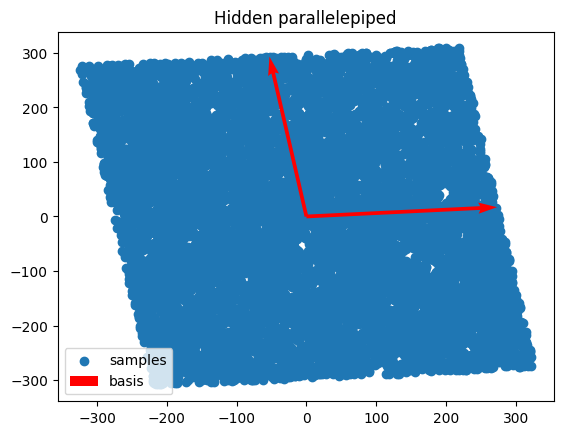
\includegraphics[width=0.7\textwidth]{hidden-parallelepiped.png}
    \caption{message-signature pairs reveal the parallelepiped spanned by the secret basis}
\end{figure}

\begin{definition}
    let $V = [\mathbf{v}_1, \mathbf{v}_2, \ldots, \mathbf{v}_n]$ be a full-rank matrix in $\mathbb{R}^{n \times n}$ and let $\mathcal{P}(V) = \{V\mathbf{x} \mid \mathbf{x} \in [-1, 1]^n\}$ denote the parallelepiped spanned by $V$. The \textbf{hidden parallelepiped problem} asks to approximate the vectors of $V$ using a polynomial-bound number of uniform samples in the parallelepiped
\end{definition}

The main algorithm for solving HPP first approximates the Gram matrix of the basis of the parallelepiped, which can then be used to approximate a linear transformation that maps the parallelepiped to a hypercube (which is a parallelepiped with an orthonormal basis). The basis of the hypercube can be approximated using a gradient descent, and the basis of the parallelpiped can be computed by inverting the hypercube transformation.

Learning the basis of a hypercube can be efficiently done through a gradient descent on the fourth moment of a uniform distribution on the hypercube:

\begin{definition}
    Given basis $V = [\mathbf{v}_1, \ldots, \mathbf{v}_n] \in \mathbf{r}^{n \times n}$, define the k-th moment of a uniform distribution on $\mathcal{P}(V)$ over a vector $\mathbf{w} \in \mathbb{R}^n$ as

    $$
    \operatorname{mom}_{V, k}(\mathbf{w}) = \exp[
        \langle \mathbf{u}, \mathbf{w} \rangle^k
    ]
    $$

    Where $\mathbf{u}$ is uniform sample from $\mathcal{P}(V)$
\end{definition}

Gradient descent on the fourth moment of the hypercube is an appropriate algorithm due to the following lemma:

\begin{lemma}
    Given basis $V = [\mathbf{v}_1, \ldots, \mathbf{v}_n] \in \mathbb{R}^{n \times n}$ of a unit hypercube, there exists a unique global minimum achieved at $\pm\mathbf{v}_1, \pm\mathbf{v}_2, \ldots, \pm\mathbf{v}_n$ and no other local minimum
\end{lemma}

\begin{algorithm}
\caption{Learning a hidden parallelepiped}
\begin{algorithmic}[1]
    \State Approximate $G^\prime \approx V^\intercal V$
    \State Compute the Cholesky factor $L$ of $G^{-1}$: $G^{-1} = LL^\intercal$
    \State Transform the parallelepiped samples into hypercube samples $\mathbf{x} \in \mathcal{P}(V) \mapsto \mathbf{x}L$
    \State Approximate the basis of the hypercube $C^\prime = [\mathbf{c}_1, \mathbf{c}_2, \ldots, \mathbf{c}_n]$
    \State Transform the hypercube basis back to parallelepiped basis $\mathbf{v} \leftarrow \mathbf{c}L^{-1}$
\end{algorithmic}
\end{algorithm}

\begin{algorithm}\label{algo-learning-hypercube}
\caption{Learning a hidden hypercube}
\begin{algorithmic}[1]
    \State Choose some initial unit vector for $\mathbf{w}$
    \While{True}
        \State Approximate the gradient $\nabla \operatorname{mom}_{V, 4}(\mathbf{w})$ of the fourth moment at $\mathbf{w}$
        \State Denote $\mathbf{w}^\prime \leftarrow \mathbf{w} - \delta \nabla \operatorname{mom}_{V, 4}(\mathbf{w})$, then normalize $\mathbf{w}^\prime$
        
        \If{$\operatorname{mom}_{V, 4}(\mathbf{w}^\prime) 
            > \operatorname{mom}_{V, 4}(\mathbf{w})$}
            \State return $\mathbf{w}$
        \Else
            \State Replace $\mathbf{w}$ with $\mathbf{w}^\prime$
        \EndIf 
    \EndWhile
\end{algorithmic}
\end{algorithm}

\subsection{Experimental results}
The GGH signature scheme and the HPP learning algorithm were implemented using Python. The matrix arithmetics, including dot products, matrix inversion, and Cholesky factorization, are all computed using numpy 1.26.2. A demo of the cryptanalysis is available on GitHub \footnote{https://github.com/xuganyu96/lattice-crypto-notes/blob/main/gghattack/demo.ipynb}.

In this implementation, the secret basis is generated using the formula $R \leftarrow kI + R^\prime$, where $R^\prime$ is uniformly sampled from $\{-l, -l + 1, \ldots, l-1, l\}^{n \times n}$, $l = 100$, and $k = \lfloor \sqrt{n} \cdot l \rceil$. Messages are uniformly sampled from $\mathbf{m} \leftarrow \{-99999, \ldots, 99999\}^n$, and signatures are computed using simple rounding algorithm $\sigma \leftarrow R \lfloor R^{-1}\mathbf{m} \rceil$. Note that we can also use nearest plane to compute the signature, although with that we will be learning the basis of the orthogonal parallelepiped spanned by $B^\ast$.

Following the recommendation of Nguyen and Regev, the rate of the gradient descent is set to $\delta = 0.7$. For initial positions of $\mathbf{w}$, we iterated through the columns of the identity matrix $I_n$, and we found that they each descended into a distinct basis. In other words, running gradient descent on each of these initial positions allowed us to approximate all secret basis vectors.

While this implementation did not recover the exact value of the secret basis, the approximated secret basis is numerically very close to the true secret basis. We meansured the quality of the basis by computing the determinant of $B^{-1}B^\prime$ where $B^\prime$ is the approximated basis: the closer this determinant is to 1, the better $B^\prime$ is an approximation of $B$.

On an M1 MacBook Air, approximating the secret basis at dimension $n = 80$ with 200000 pairs of message-signature pair could be done in only a few minutes. I could not reliably approximate secret basis of higher dimensions due to integer overflow limitations of numpy, though using C++ with appropriate big integers, the original authors were able to recover secret basis with more than 400 dimensions using 200000 samples.

\begin{figure}[h]
    \centering
    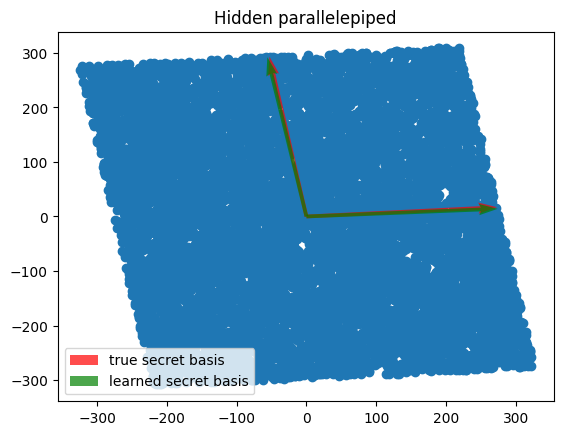
\includegraphics[width=0.7\textwidth]{learned-hpp.png}
    \caption{Recovering a strong approximation of the secret basis}
\end{figure}

\section{Conclusion and final comments}
In this project, we reviewed some fundamental results of lattices, analyzed the difficulty of hard lattice problems and the efficiency of their best known solutions. We then discussed a lattice trapdoor construction that takes advantage of an exponential gap between short basis and long basis in their ability to solve the closest vector problem, and applied the trapdoor to build a public key cryptosystem and a digital signature scheme.

Both the public-key cryptosystem and the signature scheme have been cryptanalyzed \cite{nguyen1999cryptanalysis}\cite{nguyen2006learning} in their original proposed form. However, the idea of using a pair of short and long basis to build trapdoors has been extended in later studies. Gentry, Peikert, and Vaikuntanathan developed this idea into the GPV framework\cite{gentry2008trapdoors} that later led to FALCON, a digital signature scheme that was submitted to NIST's post-quantum cryptography competition. This idea was also behind NTRUSign\cite{hoffstein2003ntrusign}, whose post-quantum variant was also submitted to NIST's post-quantum cryptography competition.

\bibliographystyle{plain}
\bibliography{./references.bib}

\end{document}